%!TEX root = paper.tex
\section{Implementation}
\label{sec:implementation}
The main jobs of InferSpark are Bayesian network construction and  code generation (\figref{fig:workflow}).
Bayesian network construction first extracts Bayesian network template from the model definition and transforms it into a
Scala class with inference and query APIs at compile time. 
%The generated class
%is compiled with normal scala part of the program 
%Then, code generation takes those as inputs and generates a Spark program which 
%including the messaging passing graph and VMP inference code. Afterwards, the generated program is executed on Spark.
Then, code generation takes those as inputs and generates a Spark program
that can generate the messaging passing graph with VMP on top.
Afterwards, the generated program would be executed on Spark.

We use the code generation approach because it enables a more flexible API
than a library. For a library, there are fixed number of APIs for user to
provide data, while InferSpark can dynamically generate custom-made APIs 
according to the structure of the Bayesian network. 
Another reason for using code generation is
that compiled programs are always more efficient than interpreted programs.

%The code generation to implement InferSpark. 
%Stage 1 constructs
%a and submitted to Spark.  
%Stage 2 performs metadata collection using Spark and generate MPG 
%construction and VMP inference code based on the meta data at run time.


%\subsection{Stage 1 Code Generation}
\subsection{Bayesian Network Construction}\label{bnc}

In this offline compilation stage, the model definition is first transformed into a Bayesian network.
We use the macro annotation, a compile-time meta programming facility of
Scala.  It is currently supported via the macroparadise plugin. After the
parser phase, the class annotated with ``{\sf @Model}'' annotation is passed from the
compiler to its transform method. InferSpark treats the class passed to it as
model definition and transforms it into a Bayesian network.

\begin{figure}[!h]
\scriptsize
	\begin{tabular}{lrl}
		ModelDef		& ::= & `@Model' `class' id \\
					&     &`(' ClassParamsOpt `)' `\{' Stmts `\}' \\
		ClassParamsOpt	& ::= & `' /* Empty */ \\
						&	| &	ClassParams \\
		ClassParams		& ::= & ClassParam  [`,' ClassParams] \\
		ClassParam		& ::= & id `:' Type \\
		Type			& ::= & `Long' | `Double' \\
		Stmts			& ::= & Stmt [[semi] Stmts]\\
		Stmt			& ::= & `val' id = Expr \\
		Expr			& ::= & `\{' [Stmts [semi]] Expr `\}' \\
						&	| & DExpr	\\
						&   | & RVExpr \\
						&	| & PlateExpr \\
						&	| & Expr `.' `map' `(' id => Expr `)'\\
		DExpr			& ::= & Literal	\\
						&   | & id \\
						&   | & DExpr (`+' | `-' | `*' | `/') DExpr \\
						&   | & (`+' | `-') DExpr	\\
		RVExpr			& ::= & `Dirichlet' `(' DExpr `,' DExpr `)' \\
						&   | & `Beta' `(' DExpr `)' \\
						&   | & `Categorical' `(' Expr `)' \\
						&   | & RVExpr RVArgList	\\
						&   | & id	\\
		RVArgList		& ::= & `(' RVExpr `)' [ RVArgList ] \\
		PlateExpr		& ::= & DExpr `until' DExpr	\\ 
						&   | & DExpr `to' DExpr	\\
						&	| & `?' \\
						&	| & id
	\end{tabular}
\caption{InferSpark Model Definition Syntax}
\label{fig:inferspark_syntax}
\end{figure}

\figref{fig:inferspark_syntax} shows the syntax of InferSpark model
definition. The expressions in a model definition is divided into 3
categories: deterministic expressions (DExpr), random variable expressions
(RVExpr) and plate expressions. The deterministic expressions include
literals, class parameters and their arithemetic operations. The random
variable expressions define random variables or plates of random variables.
The plate expressions define plate of known size or unknown size. The random
variables defined by an expression can be binded to an identifier by the value
definition. It is also possible for a random variable to be binded to multiple
or no identifiers. To uniquely represent the random variables, we assign
internal names to them instead of using the identifiers.

\begin{figure}[ht]
\centering
	\includegraphics[width=0.6\columnwidth]{figs/two_coins_internal_bn1.eps}
	\caption{Internal Rep. of Bayesian Network}
	\label{fig:two_coins_internal_bn1}
\end{figure}

Internally, InferSpark represents a Bayesian network in a tree form, where the
leaf nodes are random variables and the non-leaf nodes are plates. The edges
in the tree represent the nesting relation between plates or between a plate
and random variables. The conditional dependencies in the Bayesian network are
stored in each node.  The root of the tree is a predefined plate TOPLEVEL with
size 1.  \figref{fig:two_coins_internal_bn1} is the internal representation of
the two-coin model in \figref{fig:two_coins_bn1}, where
$r_1$, $r_2$, $r_3$, $r_4$, correspond to $\pi$, $\phi$, $z$, $x$, respectively. 
Plate 1 and Plate 2 correponds to the plates defined on lines 3--5 in
\figref{fig:two_coins_modeldef}. 

If a plate is nested within another plate,
the inner plate is repeated multiple times, in which case,
the size attribute of the plate node will be computed by summing the size of each
repeated inner plate. We call the size attribute in the tree {\em flattened size}
of a plate. For example, in \figref{fig:two_coins_nestedplates}, the flattened
size of the innermost plate around $x$ is $\sum_i N_i$.

%\begin{figure*}[!h]
%\centering
%\scriptsize
%	\begin{tabular}{|p{0.45\textwidth}|p{0.45\textwidth}|}
%		\hline
%%		ModelDef ::= @Model class id (ClassParamsOpt) \{ Stmts \} & 
%%		\begin{tabular}{l}
%%			env = {}; \\
%%			curPlate = TOPLEVEL;\\
%%			transform(ClassParamsOpt, curPlate, env); \\
%%			transform(Stmts, curPlate, env); \\
%%			genCode(TOPLEVEL, env);
%%		\end{tabular}\\\hline
%%
%%		ClassParams ::= ClassParam [, ClassParams] & 
%%		\begin{tabular}{l}
%%			transform(ClassParam, curPlate, env);\\
%%			transform(ClassParams, curPlate, env);
%%		\end{tabular} \\\hline
%%
%		ClassParam ::= id ':' Type &
%		\begin{tabular}{l}
%			env.push(id, ClassParam(Type))
%		\end{tabular} \\\hline
%%
%%		Stmts ::= Stmt [[semi Stmts]] &
%%		\begin{tabular}{l}
%%			transform(Stmt, curPlate, env);\\
%%			transform(Stmts, curPlate, env);
%%		\end{tabular} \\\hline
%%
%%		Stmt ::= val id = Expr &
%%		\begin{tabular}{l}
%%			r = eval(Expr, curPlate, env); \\
%%			env.put(id, r);
%%		\end{tabular} \\\hline
%%
%%		Expr ::= \{ [Stmts [semi]] Expr \} &
%%		\begin{tabular}{l}
%%			transform(Stmts, curPlate, env);	\\
%%			return eval(Expr, curPlate, env);	
%%		\end{tabular} \\\hline
%%
%		Expr ::= DExpr &
%		\begin{tabular}{l}
%			return DExpr;
%		\end{tabular} \\\hline
%%
%%		Expr ::= RVExpr &
%%		\begin{tabular}{l}
%%			return eval(RVExpr, curPlate, env);
%%		\end{tabular} \\\hline
%%
%%		RVExpr ::= Dirichlet(DExpr1, DExpr2) &
%%		\begin{tabular}{l}
%%			alpha = eval(DExpr1, curPlate, env);	\\
%%			dim = eval(DExpr2, curPlate, env);	\\
%%			if (alpha.type != Double || dim.tpe != Long) error;	\\
%%			r = Dirichlet(alpha, dim);	\\
%%			curPlate.addChild(Dirichlet(alpha, dim));	\\
%%			return d;
%%		\end{tabular} \\\hline
%%
%%		RVExpr ::= Beta(DExpr) &
%%		\begin{tabular}{l}
%%			alpha = eval(DExpr, curPlate, env);	\\
%%			if (alpha.type != Double) error; \\
%%			r = Dirichlet(alpha, 2); \\
%%			curPlate.addChild(r); \\
%%			return r;
%%		\end{tabular} \\\hline
%%
%		RVExpr ::= Categorical(Expr) &
%		\begin{tabular}{l}
%			p = eval(Expr, curPlate, env); \\
%			if (p.type != DoubleVector) error;\\
%			if (p.isRV \&\& p is not Dirichlet) error;\\
%			r = Categorical(p); \\
%			curPlate.addChild(r); \\
%			return r;
%		\end{tabular} \\\hline
%
%		RVExpr ::= RVExpr RVArgList &
%		\begin{tabular}{l}
%			(r, plate) = eval(RVExpr, curPlate, env);\\
%			argList = eval(RVArgList, curPlate, env); \\
%			if (argList.length != r.depth - plate.depth) error;\\
%			if (argList.find(!conjugate to r || type is not Long)) error;\\
%			return Mixture(r, plate, argList);
%		\end{tabular} \\\hline
%%
%%		RVExpr ::= id &
%%		\begin{tabular}{l}
%%			return env.get(id);
%%		\end{tabular} \\\hline
%%
%%		PlateExpr ::= DExpr1 until DExpr2 &
%%		\begin{tabular}{l}
%%			low = eval(DExpr1, curPlate, env);\\
%%			high = eval(DExpr2, curPlate, env); \\
%%			p = Plate(ExclusiveRange(low, high)); \\
%%			curPlate.addChild(p);
%%			return p;
%%		\end{tabular} \\\hline
%%
%%		PlateExpr ::= DExpr1 to DExpr2 &
%%		\begin{tabular}{l}
%%			low = eval(DExpr1, curPlate, env);\\
%%			high = eval(DExpr2, curPlate, env); \\
%%			p = Plate(InclusiveRange(low, high)); \\
%%			curPlate.addChild(p);
%%			return p;
%%		\end{tabular} \\\hline
%%
%		PlateExpr ::= ? &
%		\begin{tabular}{l}
%			p = Plate(UnknownRange); \\
%			curPlate.addChild(p);
%			return p;
%		\end{tabular} \\\hline
%
%		Expr ::= Expr1.map(id => Expr2) &
%		\begin{tabular}{l}
%			left = eval(Expr1, curPlate, env);\\
%			if (left is plate) \{\\
%				r = eval(Expr2, left, env);\\
%				return (r, left); \\
%			\} else if (left = (r1, plate)) \{ \\
%				env.put(id, (r1, plate(r1)));\\
%				r2 = eval(Expr2, plate, env);\\
%				env.pop(id);\\
%				return (r2, plate);\\
%			\} else error;
%		\end{tabular}\\\hline
%
%	\end{tabular}
%	\caption{Transformation Rules}
%	\label{fig:transformation_rules}
%\end{figure*}

InferSpark recursively descends on the abstract syntax tree (AST) of the model definition to construct
the Bayesian network.   In the
model definition, InferSpark follows the normal lexical scoping rules.
%\figref{fig:transformation_rules} shows part of the transformation rules of each
%syntax. ``transform(ast, curPlate, env)'' transforms non-expression parts while
%``eval(ast, curPlate, env)'' transforms expression and result the evaluation result.
InferSpark evaluates the expressions to one of the following three results
\begin{itemize}
	\item a node in the tree
	\item a pair $(r, \textrm{plate})$ where $r$ is a random variable node
		and plate is a plate node among its ancestors, which represents all
		the random variables in the plate
	\item a determinstic expression that will be evaluated at run time
\end{itemize}
%When defining the random variables, InferSpark also checkes the conjugacy
%constraints of the Bayesian network.

At this point, apart from constructing the Bayesian network representation, 
InferSpark also generates the code for metadata collection, a module used in 
stage 2. For each random variable name bindings, a singleton interface object 
is also created in the resulting class. 
The interface object provides ``{\sf observe}'' and ``{\sf getResult}'' API for later use.

%Value definitions ``val'' id ``='' Expr has two functionalities in InferSpark.
%First, it binds the result of the evaluation result of an expression to an
%identifier. Secondly, it declares an interface singleton
%object for the random variable that the right hand side evaluates to.
%For value definitions that inside a plate, the singleton object
%is nested inside the outer object at definition site. For example, 
%
%\begin{figure}[h]
%\begin{lstlisting}[numbers=none]
%	val trial = ?.map{_ =>
%		val z = Categorical(pi)
%		val x = ?.map{_ => Categorical(phi(z))
%	}
%\end{lstlisting}
%\caption{Path Of Interface}
%\label{sec:path}
%\end{figure}
%defines multiple trials in which we first choose a coin and then flip it for
%multiple times. The interface singleton generated is ``trial.z'' ``trial.x''.
%To implement this feature, Inferspark calculates the path, a list of
%identifiers in the chain of value definitions. For ``z'' and ``x'', the path
%are [``trial'', ``x''] and [``trial'', ``z'], respectively.
%
%In Inferspark, the Bayesian network is represented as a tree.
%\figref{fig:two_coins_internal_bn1} is the internal representation of the
%Bayesian network of two-coin model, where $r_1$, $r_2$, $r_3$, $r_4$,
%correspond to pi, phi, z, x, respectively. The non-left nodes of the tree is
%always plates while the leaf nodes are either random variable or empty plate.
%The root is a predefined plate with constant size 1 called TOPLEVEL. The depth
%of TOPLEVEL is 0. Child node has depth one larger than parent (e.g. $r_1$,
%plate 1 and 2 are of depth 1, the others are of depth 2).
%
%An expression evaluates to one of the following three:
%\begin{itemize}
%	\item a node in the tree
%	\item a pair $(r, \textrm{plate})$ where $r$ is a random variable node
%		and plate is a plate node among its ancestors
%	\item a determinstic expression that will be evaluated at run time
%\end{itemize}
%and is divided into 3 categories: deterministic expression, random variable
%expression and plate expression.
%
%Deterministic expression can be literals of Long and Double, class parameters
%or arithmetic operations on deterministic expressions. It evaluates to itself.
%
%Plate expression includes exclusive range (e.g. ``0 until 1''), inclusive
%range (e.g. ``0 to 1'') and unknown range ``?''. Plate expressions always
%create new plates. Plate expression evaluates to the node of the new plate.
%
%Random variable expression includes primitive random distributions and
%mixture. The primitive random distributions we currently support are Beta,
%Dirichlet and categorical distribution. The parameters of the distributions
%can be a deterministic value or a random variable node. The mixture expression
%is of form ``id(id1)(id2)...(idn)'', where id evaluates to a pair $(r,
%\textrm{plate})$ where the depth of plate is $n$ smaller than that of $r$.
%`id1'' to ``idn'' evaluates to random variable nodes, which selects the
%corresponding component. We have an restriction that ``id1'', ... ``idn'' are
%independent, which we may remove in the future work.
%
%``map'' call can be applied to a plate node plate or a pair $(r,
%\textrm{plate})$. When it is applied to a plate node, the formal parameter of
%the anonymous function argument is ignored. When it is applied to a pair $(r,
%\textrm{plate})$, the formal parameter of the anonymous function is binded to
%the $r$ if $r$'s parent in the tree is plate, or another pair ($r$, plate')
%where plate' is child of plate and is ancestor of $r$. For both cases, the
%body of the anonymous function can be a sequence of value definitions followed
%by an expression. The plate or random variables defined inside the body is put
%in plate. If the body expression evaluates to a random variable node $r'$ or a
%pair $(r', \textrm{plate}')$, the ``map'' evaluates to ($r$, plate).  
%
%For example, line 4 first defines plate 2 with unknown size in the TOPLEVEL.
%Then it applies ``map'' to plate 2. Inside the anonymous function, a
%Categorical variable $r_3$ is defined and put in plate 2. The ``map''
%evaluates to a pair $(r_3, \textrm{plate 2})$, which is binded to identifier
%z. On line 5, the outermost identifier z evaluates to a pair $(r_3,
%\textrm{plate 2})$.  When ``map'' is applied to it, the formal parameter ``z''
%is binded to $r_3$. The anonymous function body defines a categorical mixture
%$r_4$ and``map'' evaluates to $(r_4, \textrm{plate 2})$. Finally, $(r_4,
%\textrm{plate 2})$ is binded to the identifier x.
%
%After the construction of the Bayesian network, Inferspark generates code that
%implements the metadata collection (e.g. ``observe'') and parts of the second
%stage compilation. These parts depends on the structure of the Bayesian
%network thus must be generated. For example, x in the two-coin model is a
%Categorical random variable inside a plate size so the observed data type is
%``RDD[Long]''. ``trial.x'' in the \figref{fig:path} has two nested plates
%around it, so the observed data type is ``RDD[Array[Long]]''. Parts that do
%not depend on the structures are put into the precompiled runtime libarary of
%Inferspark. The implementation of both parts are discussed in next subsection.

\subsection{Code Generation}

Code generation happens at run time. It is divided into 4 steps: metadata
collection, message annotation, MPG construction code generation and inference
execution code generation.

Metadata collection aims to collect the values of the model parameters,
check whether random variables are observed or not, the flattened sizes of the plates.
These metadata can help to 
assign VertexID to the vertices on the message passing graph.  
%If a plate is the innermost plate that a random variable is in, the flat size of
%the plate is defined as the number of this random variable. For example, the
%flat size of plate 2 in \figref{fig:two_coins_internal_bn1} is the number of
%outcomes $x$ or the number of the random variable $z$.  
After the flattened sizes of plates are calculated, we can assign VertexIDs to the
vertices that will be constructed in the message passing graph. Each random
variable will be instantiated into a number of vertices on the MPG where the
number equals to the flattened size of its innermost plate. The vertices
of the same random variable are assigned consecutive IDs. For example, $x$ may
be assigned ID from $0$ to $N-1$. The intervals of IDs of random variables in
the same plate are also consecutive. A possible ID assignment to $z$ is $N$ to
$2N - 1$. Using this ID assignment, we can easily i) determine which random
variable the vertex is from only by determining which interval the ID lies
in; ii) find the ID of the corresponding random variable in the same plate by
substracting or adding multiples of the flattened plate size (e.g. if $x_i$' ID is
$a$ then $z_i$'s ID is $a + N$).

Message annotation aims to annotate the Bayesian Network Template from the previous stage (Section \ref{bnc})
with messages
to be used in VMP algorithm.  The annotated messages are stored in the form of
AST and will be incorporated into the the generated code, output of this stage. 
The rules of the messages to annotate are predefined according to the
derivation of the VMP algorithm.
%The messages between different types of random variables without mixture can
%be created by looking up in a table. For a mixture variable, the message from
%it is composed from basic messages in the table. 
%\KZ{Where is the table, what
%is it like?}
%
%We also need to generate two additional functions for each random variable: a
%message merge function and a vertex update function. 
%\KZ{Don't understand:
%The messages are first
%sent to the vertices to update and merged on the fly, then joined with the
%original vertices to apply the update.}  
After the messages are generated, we
generate for each type of random variable a class with the routines for
calculating the messages and updating the vertex. 

The generated code for constructing  the message passing graph requires  building a VertexRDD
and an EdgeEDD. The VertexRDD is an RDD of VertexID and vertex attribute pairs.
Vertices of different random variables
are from different RDDs (e.g., {\sf v1}, {\sf v2}, and {\sf v3} in \figref{fig:two_coins_mpg_constr_code})
and have different initialization methods.
For unobserved random variables, the source can be any RDD that has the same
number of elements as the vertices instantiated from the random variable. For
observed random variables, the source must be the data provided by the user. If
the observed random variable is in an unnested plate, the vertex id can be
calculated by first combining the indices to the data RDD then adding an offset.

One optimization of constructing the EdgeRDD is to \emph{reverse the edges}.
If the code generation process generates an EdgeRDD in straightforward manner,
the {\sf aggregateMessages} function 
has to scan all the edges 
to find edges whose destinations are of $v$ type
because GraphX indexes the \emph{source} but not the \emph{destination}.
Therefore, when constructing the EdgeRDD, we generate code that reverses the edge
so as to enjoy the indexing feature of GraphX.
When constructing the graphs,
we also take into account the graph partitioning scheme 
because that has a strong influence on the performance.
We discuss this issue in the next section.


The final part is to generate the inference execution code that implements the
iterative update of the VMP algorithm. 
We aim to generate code that updates each vertex in the
message passing graph at least once in each iteration. 
As it is safe to update vertices that do not
have mutual dependencies, i.e., those who do not send messages to one another,
we divide each iteration into substeps.
Each substep updates a portion of the
message passing graph that does not have mutual dependencies. 

A substep in each iteration consists of two GraphX operations:
{\sf aggregateMessages} and {\sf outerJoinVertices}. Suppose {\sf g} is the message passing
graph, the code of a substep is:
\begin{lstlisting}
val prevg = g
val msg = g.aggregateMessages(sendMsg, mergeMsg, TripletFields)
g = g.outerJoinVertices(msg)(updateVertex).persist()
g.edges.count()
prevg.unpersist()
\end{lstlisting}

The RDD {\sf msg} does not need to be cached because it is only used once. But
the code generated has to cache the graph {\sf g} because the graph is used 
twice in both {\sf aggregateMessages} and {\sf outerJoinVertices}. However, only caching it is not
enough, the code generation has to include a line like 4 above to activate the caching process.
Once {\sf g} is cached, code generation evicts the previous (obsolete) graph {\sf prevg} from the cache.
To avoid the long lineage caused by iteratively updating message passing graph, which will overflow the heap space of the drive,
the code generation process also adds a line of code to checkpoint the graph to HDFS 
every $k$ iterations.

\subsection{Execution}

The generated code at run time are sent to the Scala compiler. The resulting
byte code are added to the classpath of both the driver and the workers. Then
InferSpark initiates the inference iterations via reflection invocation.

%\subsection{Optimizations}
%
% 
%
%Some part of messages may be wasted because the receiver does not need it. For
%example, we only send the component in a vector message that is actually
%needed by the receiver. The index of the needed component is stored as an Edge
%attribute.
%
%We also constrain the {\sf sendMsg} function of each vertex to use only the
%attribute of the sender. This allows the {\sf aggregateMessages} to use only one end of
%the edge triplet. In this case, only the used side of an edge will be
%replicated in the edge partition, which reduces the memory footprint.
%
%\KZ{Is the following too much detail? and the optimization doesn't seem to be too big.
%One thing reminds me, do we have experiments that show the results with and without
%these optimizations?}
%We use {\sf aggregateMessages} to pull messages from multiple senders. The senders
%may have edges that do not point to the receiver we want to update in the
%substep, but all the edges pointing to the receiver have some message to send.
%In this case, it is more efficient to do an index scan on the all the edges
%destined at the vertices that we want to update and then apply the {\sf sendMsg}
%function because it scans fewer edges. However, the GraphX only builds index
%on the source end in each edge partitions. To utilize the index, we reverses
%all the edges so that the receiver of the messages is the source end of the
%edges. This optimization is useful because in each substep we usually do not
%pull messages from all the vertices. Another issue in utilizing the index is
%that we have to apply an activeSet and also an activeDirection to specify the
%sources and direction of edges to filter. In this case, we want to filter out all
%the vertices that are not updated in this iteration and we only need outgoing
%edges. The public API in GraphX does not support it but the internal API
%{\sf aggregateMessageWithActiveSet} does implement the feature. We case the graph to
%GraphX's internal implementation to use the feature.
%
%Next optimization is related to {\sf outerJoinVertices}. When GraphX does outerJoin,
%it first performs the join on the vertices. Then it ships the updated vertices
%to edge partitions where the vertex is needed. Howvever, the incremental
%update of edge partitions is only allowed when the two joined VertexRDD has
%the same vertex attribute type. In our case, the incremental update requires
%the messages and vertices to be the same type. While it is tedious for human
%to code, we generate code so that vertices and messages share the common base
%type and insert cast when necessary. This fools the {\sf outerJoinVertices} to apply
%incremental update.

\subsection{Discussion on Partitioning Strategies}

\begin{figure}[h]
	\includegraphics[width=0.45\textwidth]{figs/mixture_mpg.eps}
	\caption{Message Passing Graph of a Mixture Model}
	\label{fig:mixture_mpg}
\end{figure}

GraphX adopts a vertex-cut partitioning approach.
The vertices are replicated in edge partitions instead of edges being replicated in vertex
partitions. 
%This replication creates a triplet view, which is a 3-tuple of
%source vertex, edge and destination vertex. The triplet view is not
%materialized until referenced. For our purpose, only {\sf aggregateMessages}
%use the destination end of the triplet view, so only the destination of each
%edge is replicated in the edge partitions. We want to minimize the number of
%replications so that outerJoin is more efficient. 
The four built-in partition
strategies in GraphX are: 
EdgePartition1D (1D),
EdgePartition2D  (2D),
RandomVertexCut (RVC), and
CanonicalRandomVertexCut (CRVC).
In the following, we first show that these general 
partitioning strategies perform badly for the VMP algorithm on MPG.
Then, we introduce our own partitioning strategy.

\figref{fig:mixture_mpg} shows a more typical message passing graph of a
mixture model instead of the toy two-coin model that we have used so far. $N$
is the number of $x$ and $z$, $K$ is the number of $\phi$, $D$ is the number
of $\theta$. Typically, $N$ is very large because that is the data size (e.g.,
number of words in LDA), $K$ is a small constant (e.g., number of topics in
LDA), and $D$ could be a constant or as large as $N$ (e.g., number of
documents in LDA). 


EdgePartition1D essentially is a random partitioning strategy, except that it
co-locates all the edges with the same source vertex. Suppose all the edges from
$\phi_k$ are assigned to partition $k$. Since there's an edge from $\phi_k$ to
each one of the $N$ vertices $x$, partition $k$ will have the replications
of all $x_1, x_2, \ldots, x_N$. In the best case, 
edges from different $\phi_k$ are assigned to different
partitions. Then the largest edge partition still have at least $N$ vertices.
When $N$ is very large, the largest edge partition is also very large, which
will easily cause the size of an edge partition to exceed the RDD block size limit. However,
the best case turns out to be the worst case 
when it comes to the number of vertex replications
because it actually replicates the size $N$ data $K$ times, which is
extremely space inefficient. The over-replication also incurs large amount of
shuffling when we perform outer joins because each updated vertex has to
be shipped to every edge partition, prolonging the running time. 

We give a more formal analysis of the number of vertices in the largest edge
partition and the expected number of replications of $x_i$ under
EdgePartition1D. As discussed above, there's at least one edge partition that
has replications of all the $x_i$'s. 
Observe that the graph has an upper bound of
$3N + K$ vertices, so the number of vertices in the largest edge partition is
$O(N)$. Let $N_{x_i}$ be the number of replications of $x_i$, then the expected
number of replication of $x_i$ is 
\begin{align*}
	E[N_{x_i}] &= M(1 - (1 - \frac{1}{M})^{K+1}) \\
		&= \left\{
			\begin{array}{ll}
				(K + 1) + o(1) & K = O(1) \\
				M + o(1) & K = O(M) 
			\end{array}
		\right.%}
\end{align*}



%first introduction 
%then analysis
\begin{figure}[h]
	\centering
	\includegraphics[scale=0.3]{figs/2dhash.eps}
	\caption{EdgePartition2D.  Each grid is a partition. The possible partitions in which $x_i$ is
	replicated is shaded}
	\label{fig:2dhash}
\end{figure}

EdgePartition2D evenly divides the adjacency matrix of the graph into $\sqrt{M}
\times \sqrt{M}$ partitions. The vertices are uniformly distributed along the
edges of the adjacency matrix by hashing into $\sqrt{M}$ buckets. The upper
bound of the number of replications of a vertex $x_i$ is $\sqrt{M}$ because all
the edges that point to it are distributed to at most $\sqrt{M}$ partitions
in shown as \figref{fig:2dhash}.  Meanwhile, there are $K+1$
edges pointing to $x_i$, so the number of replications of $x_i$ cannot exceed
$K+1$ as well. Therefore, the upper bound of replications of $x_i$ is actually
$\min(K+1, \sqrt{M})$. On the other hand, suppose each of the $\phi_k$ is
hashed to different bucket and $N$ $x$'s are evenly distributed into the
$\sqrt{M}$ buckets, then the number of largest partition is at least
$\frac{N}{\sqrt{M}}$, which is still huge when the average number of words per
partition is fixed. Following is the formal analysis of the EdgePartition2D.

Let $B$ be an arbitrary
partition in the dark column on \figref{fig:2dhash}.
Let $Y_{x_i, B}$ be the indicator variable for the event that $x_i$ is replicated in 
Then the expectation of $Y_{x_i, B}$ is
\begin{align*}
	E[Y_{x_i, B}] &= 1 - (1 - \frac{1}{\sqrt{M}})^{K+1} \\
\end{align*}

The number of vertices $N_B$ in the largest partition $B$ is at least the expectation
of the number of vertices in a partition, which is also at least the
expectation of the number of $x_i$ in it:
\begin{align*}
	E[N_{B}] &= \sum_{v} E[Y_{v, B}] \\
		&\ge \frac{N}{\sqrt{M}} E[Y_{x_i, B}]	\\
		& = \left\{
				\begin{array}{ll}
					(K + 1)\eta	+ o(1) & K = O(1) \\
					\sqrt{M}\eta + o(1) & K = O(M) 
				\end{array}
			\right.%}
\end{align*}

The expected number of replications of $x_i$ is
\begin{align*}
	E[N_{x_i}] &= \sqrt{M}E[Y_{x_i, B}] \\
		&= \left\{
			\begin{array}{ll}
				(K + 1) + o(1) & K = O(1) \\
				\sqrt{M} + o(1) & K = O(M) 
			\end{array}
		\right.%}
\end{align*}


%
RandomVertexCut (RVC) uniformly assigns each edge to one of the $M$
partitions. The expected number of replications of $x_i$ tends to be $O(K)$
when $K$ is a constant and tends to be $O(N)$ when $K$ is proportional to the
number of partitions. The number of vertices in the largest partition is also
excessively large. It is $O(K\frac{N}{M})$ when K is a constant and $O(N)$
when $K$ is proportional to the number of partitions.  CanonicalRandomVertexCut
assigns two edges between the same pair of vertices with opposite directions
to the same partition. For VMP, it is the same as RandomVertexCut since only
the destination end of an edge is replicated. For example, if $x_i$ has $K +1$
incoming edges, then the probability that $x_i$ will be replicated in a
particular partition is independent from whether edges in opposite
direction are in the same partition or randomly distributed. Therefore 
CRVC will have the same result as RVC.  
\tabref{tab:max_v_per_edge_part_O1} and
\tabref{tab:max_v_per_edge_part_OM} summarize the comparison of different
partition strategies.

InferSpark's partitioning strategy is actually tailor-made for VMP's message passing graph.
The intuition is that the MPG has a special structure.
For example, in \figref{fig:mixture_mpg},
we see that the MPG essentially has $D$ ``independent'' trees rooted at $\theta_i$,
where the leaf nodes  are $x$'s and they form a complete bipartite graph with all $\phi$'s.
In this case, one good partitioning strategy is to form $D$ partitions, 
with each tree going to one partition and the $\phi$'s getting replicated $D$ times.
We can see that such a partition strategy incurs no replication on $\theta$, $z$, and $x$,
and incurs $D$ replications on $\theta$.

Generally, our partitioning works as follows: Given an edge, we first determine
which two random variables (e.g. $x$ and $z$) are connected by the edge. It is
quite straightforward because we assign ID to the set of vertices of the same
random variable to a consecutive interval. We only need to look up which
interval it is in and what the interval corresponds to. Then we compare the
total number of vertices correponding to the two random variables and choose
the larger one. Let the Vertex ID range of the larger one to be $L$ to $H$. We
divide the range from $L$ to $H$ into $M$ subranges. The first subrange is $L$
to $L + \frac{H-L+1}{M}$; the second is $L + \frac{H-L+1}{M} + 1$ to $L +
2\frac{H-L+1}{M}$ and so on. If the vertex ID of the edge's chosen vertex falls
into the $m^{th}$ subrange, the edge is assigned to partition $m$.

In the mixture case, at least one end of every edge is $z$ or $x$. Since
the number of $z$'s and $x$'s are the same, 
each set of edges that link to the $z_i$ or $x_i$ with 
the same $i$ are co-located. This guarantees that $z_i$
and $x_i$ only appears in one partition. All the $\phi_k$'s are replicated in each
of the $M$ partitions as before. The only problem is that many $\theta_j$ with
small $N_j$ could be replicated to the same location. In the worst case, the
number of $\theta$ in one single partition is exactly $\eta$. However, it is
not an issue in that case because the number of vertices in the largest
partition is still a constant $3\eta + K$. It is also independent from whether $K
= O(1)$ or $K = O(M)$.


\begin{table}[h]
	\centering
	\caption{Analysis of Different Partition Strategies When $K = O(1)$}
	\label{tab:max_v_per_edge_part_O1}
	\begin{tabular}{lll}
		\hline
		Partition Strategy & $E[N_{x_i}]$ & $E[N_B]$\\\hline\hline
		1D & $O(K)$ & $O(N)$ \\\hline
		2D & $O(K)$ & $O(K\frac{N}{M})$ \\\hline
		RVC & $O(K)$ & $O(K\frac{N}{M})$ \\\hline
		CRVC & $O(K)$ & $O(K\frac{N}{M})$ \\\hline
		{\bf InferSpark} & 1 & $3\frac{N}{M}+1$ \\\hline
	\end{tabular}
\end{table}

\begin{table}[h]
	\centering
	\caption{Analysis of Different Partition Strategies When $K = O(M)$}
	\label{tab:max_v_per_edge_part_OM}
	\begin{tabular}{lll}
		\hline
		Partition Strategy & $E[N_{x_i}]$ & $E[N_B]$\\\hline\hline
		1D & $O(M)$ & $O(N)$ \\\hline
		2D & $O(\sqrt{M})$ & $O(\sqrt{M}\frac{N}{M})$ \\\hline
		RVC & $O(M)$ & $O(N)$ \\\hline
		CRVC & $O(M)$ & $O(N)$ \\\hline
		{\bf InferSpark} & 1 & $3\frac{N}{M}+1$ \\\hline
	\end{tabular}
\end{table}

%%%%%%%%%%%%%%
%
%If there is an edge between two vertices, then there is also one in the
%opposite direction.  The number of edges between $\theta$ and $z$ is always
%$N$. $z$ and $x$ are one-to-one correspondence. 
%$x$ and $\phi$ form a full bipartite graph.
%
%
%When the data size $N$ increases, it is also natural to scale up the cluster
%size. Let $M$ be the number of partitions that the edges and vertices will be
%partitioned into. We assume that the average number of data points in each
%vertex partition $\eta = \frac{N}{M}$ is a large constant.  In the rest of
%of this subsection, we denote the degree and in-degree of a vertex $v$ in the
%MPG as $D(v)$ and $D_{in}(v)$.
%Let $B_1, B_2, \ldots, B_M$ be the $M$ partitions and
%$N_{B_m}$ be the number of vertices replicated in partition $B_m$. \KZ{why
%replicated in partition Bm? I thought all the vertices are replicated in a
%partition anyway?} We also write $N_{x, B_m}$ to represent the number 
%of $x$'s in partition $B_m$.  For a
%vertex $v$ in the graph, We define $Y_{v,B_m}$ to be the indicator variable of
%the event that vertex $v$ is in $B_m$. Let $N_{v}$ be the number of
%replications of the vertex $v$. We analyze the lower bound of the maximum
%number of verticies replicated in a partition $\max{N_{B_M}}$ and the expected
%number of replications of $x_i$ $E[N_{x_i}]$ for two cases where $K =
%O(1)$ and $K = O(M)$.
%
%
%We first analyze the 2D hash partitioning \cite{graphX} that comes with GraphX. The
%2D hash partitioning evenly divide the adjacency matrix of the graph into
%$\sqrt{M} \times \sqrt{M}$ partitions. The vertices are uniformly 
%distributed along the edges of the adjacency matrix by hashing into $\sqrt{M}$
%buckets. In the general case where both source and destination of an edge can be
%replicated, the upper bound of replication of a vertex $v$ is $\min(2\sqrt{M}
%- 1,D(v))$ (\figref{fig:2dhash}). In our VMP implementation, the upper bound is
%$\min(\sqrt{M}, D_{in}(v))$ because only the destination end of an edge could
%be replicated. Due to this upper bound, 2D hash partitioning is much better
%than the other three when $K = O(M)$ and it at least the same when $K = O(1)$.
%However, we show in the following that the upper bound can be attained in both
%cases.
%
%Let $v$ be an arbitrary vertex in the graph and $B_m$ be an arbitrary
%partition in the dark column on the right hand side of \figref{fig:2dhash}.
%The probability that $v$ is replicated in $B_m$ or the expectation of $Y_{v,
%B_m}$ is
%\begin{equation}
%	E[Y_{v, B_m}] = p(Y_{v, B_m}) = 1 - (1 - \frac{1}{\sqrt{M}})^{D_{in}(v)}
%\end{equation}
%Substituting $x_i$ for $v$, we get
%\begin{align*}
%	E[Y_{x_i, B_m}] &= 1 - (1 - \frac{1}{\sqrt{M}})^{K+1} \\
%\end{align*}
%
%Hence, the expected number of vertices replicated in the partition $B_{m}$ is
%at least the expectation of the number of $x_i$ in it,
%\begin{align*}
%	E[N_{B_m}] &= \sum_{v} E[Y_{v, B_m}] \\
%		&\ge \frac{N}{\sqrt{M}} E[Y_{x_i, B_m}]	\\
%		& = \left\{
%				\begin{array}{ll}
%					(K + 1)\eta	+ o(1) & K = O(1) \\
%					\sqrt{M}\eta + o(1) & K = O(M) 
%				\end{array}
%			\right.%}
%\end{align*}
%
%The expected number of replications of $x_i$ is
%\begin{align*}
%	E[N_{x_i}] &= \sqrt{M}E[Y_{x_i, B_m}] \\
%		&= \left\{
%			\begin{array}{ll}
%				(K + 1) + o(1) & K = O(1) \\
%				\sqrt{M} + o(1) & K = O(M) 
%			\end{array}
%		\right.%}
%\end{align*}
%
%From above we find that each mixture variable $x_i$'s number of replication
%reaches the upper bound in expectation. The largest partition size grows
%propotional to $K + 1$ when $K = O(1)$ and $\sqrt{M}$ when $K = O(M)$.
%
%
%Next, we analyze the 1D hash partitioning. The 1D hash partitioning strategy
%uniformly assigns edges to each partition according to the hash value of the
%source vertex ID. Since $\phi_k$ in the graph has $N$ edges that link to each
%of the $x_i$, the $N$ edges are hashed to the same partition. So the maximum
%size of partition is at least $N = M\eta$ in all cases. This is essentially
%the worst case that could happen because we replicate at least one third of
%the graph in a single partition.
%The expected number of replications of $x_i$ is 
%\begin{align*}
%	E[N_{x_i}] &= M E[Y_{x_i, B_m}] \\
%			&= M (1 - (1 - \frac{1}{M})^{K+1}) \\
%			&= \left\{
%				\begin{array}{ll}
%					K+1 + o(1) & K = O(1) \\
%					O(M) & K = O(M)
%				\end{array}
%			\right.%}
%\end{align*}
%This number is the same as 2D when $K = O(1)$. When $K = O(M)$, it is much worse the 2D
%because it increases linearly.
%
%
%\begin{figure}[h]
%	\centering
%	\includegraphics[scale=0.4]{figs/mixture_part_mpg.eps}
%	\caption{Part of the Message Passing Graph of Mixture Model}
%	\label{fig:mixture_part_mpg}
%\end{figure}

%The reason why the built-in partition strategy fails is that they randomly
%distribute the edges, which causes over-replication of the vertices. Consider
%part of the graph in \figref{fig:mixture_part_mpg}. An intuitive partition
%strategy is to colocate all the edge shown in the part. Then we only have one
%replications of $\theta$, $x$ and $z$, while all the $\phi$'s are replicated
%in every one of the $M$ partitions. The replication of $\phi$ is okay because
%$K$ is much smaller than $N$. Under the intuitive partition strategy, the
%shuffling of the largest part of the graph $x$, $z$ is minimal while the
%smaller part is broadcasted to each partition. If $N_1 = N_2 = \ldots = N_D =
%\frac{N}{D}$, then each partition roughly have the same number of vertices
%$\frac{D}{M} + 2\eta + K$, regardless of $K = O(1)$ or $K = O(M)$. However,
%the intuitive strategy performs bad when the data is skewed. For example, when
%$N_1 = N - D, N_2 = \ldots = N_D = 1$, the largest partition has at least
%$2(N-D) + K + 1$ vertices, which is as bad as 1D partition strategy.
%
%\KZ{Is the following paragraph InferSpark partitioning strategy?}
%Based on the observation, we give InferSpark partitioning strategy that evenly
%distribute the vertices while preserving the structure of the graph. 



%\figref{fig:max_v_per_edge_part_O1} and \figref{fig:max_v_per_edge_part_OM}
%shows the comparison of different partition strategies. RVC refers to Random
%Vertex Cut and CRVC refers to Canonical Random Vertex Cut. RVC uniformaly
%distribute the edges according to the hash of both source and destination ID.
%CRVC chooses a canonical direction when hashing the edges so that edges in
%opposite directions are colocated. The two strategy are the same in our case.
%The probability of a vertex replicated to a partition is the same because we
%only replicate the destination. From the two tables, we find that our
%partition strategy is the only one that is irrelevant to $K$ and the number of
%partitions $M$, and data size $N$ as long as the average number of data points
%in each partition is a constant, so it will scale better than the built-in
%partition strategies. \KZ{What exactly is the InferSpark's partition strategy.
%Did I miss something?}

%--------------------------------------------------------------------------
%	BELOW ME ARE NOT REWRITTEN
%--------------------------------------------------------------------------
%\begin{figure*}[!ht]
%	\centering
%\begin{tabular}{l*{5}{p{50pt}}}
%	\hline
%	Name & InferSpark & 2D & 1D & RVC & CRVC \\\hline
%	$E[N_{x_i}]$ & $1$ & $O(K)$ & $O(K)$ &
%	$O(K)$ & $O(K)$ \\\hline
%	$\max N_{b_m}$ & $2\eta + 1$ & $O(K\eta)$ &
%	$O(p\eta)$ & $O(K\eta)$ & $O(K\eta)$  \\\hline
%\end{tabular}
%\caption{Comparison of maximum number of vertices per edge partition when $K = O(1)$}
%\label{fig:max_v_per_edge_part_O1}
%\end{figure*} 
%
%\begin{figure*}[!ht]
%\begin{tabular}{l*{5}{p{50pt}}}
%	\hline
%	Name & InferSpark & 2D & 1D & RVC & CRVC \\\hline
%	of Replications of $x_i$ & $1$ & $O(\sqrt{p})$ &
%	$O(p)$ & $O(p)$ & $O(p)$ \\\hline
%	$\max $ \#vertices per Partition & $2\eta + 1$ &
%	$O(\sqrt{p}\eta)$ & $O(p\eta)$ & $O(p\eta)$ & $O(p\eta)$ \\\hline
%\end{tabular}
%\caption{Comparison of maximum number of vertices per edge partition when $K = O(p)$}
%\label{fig:max_v_per_edge_part_Op}
%\end{figure*}
%
%The mixture model is common in various models (e.g. the two-coin, GMM, LDA)
%and is often the bottleneck of scalability. Without loss of generality, we
%consider the mixture of $K$ Categorical distributions there are $N$ such
%mixture random variables. Denote the parameters of each Categorical
%distribution as $\phi_k$, which has Dirichlet priors. The mixture random
%variables are denoted as $x_i$ and the corresponding choice mixture is denoted
%as $z_i$. In the two-coin model, $K = 2$. In the LDA model, $K$ both
%constants.  We consider two situations: $K = O(1)$ and $K = cp$, where $c$ is a
%small constant.  We ignore other parts of the model because they only takes up
%a small fraction of the graph compared to $x$ and $z$. 
%
%Let $p$ be the number of partitions of the graph. It is reasonable to assume
%that the average number of raw data of $x$ per partition $\eta = \frac{N}{p}$
%is a constant because we would scale up the cluster size when the data size
%increases. and we
%analyze Inferspark's partition strategies and 4 GraphX built-in partition
%strategies. Our VMP implementation only uses the destination end of the
%triplet view so only the destination end is replicated in the edge partitions.

%Our partition strategy evenly distribute the edges between two random
%variables in the Bayesian network by the end whose multiplicity is larger. In
%the mixture case, $N >> K$, so the edges between $x$ and $\phi$ are
%partitioned by $x$'s id. The first $\eta$ $x$'s edges from and to $\phi$ are
%located in partition 2, the second $\eta$ $x$'s edeges are in partition 2 and
%etc. The $x_i$ and $z_i$ are one-to-one so the edge between $x_i$ and $z_i$
%are colocated with edges between $x_i$ and $\phi$.
%\figref{fig:inferspark_partitionstrategy} shows our partition strategy. Under
%this partition strategy, the number of replication of x and z is 1 because all
%the edges with destination $x_i$ and $z_i$ are in the same partition. The
%smaller part $\phi$ are replicated in each partition. The number of vertices
%per edge partition is $2\eta + K$. This is constant regardless of whether $K
%= O(1)$ or $K = O(p)$ and increase of datasize or number of partitions.
%
%The built-in 2D hash paritition strategy (EdgePartition2D) \cite{graphX}
%divides each side of the adjacency matrix into $\sqrt{p}$ equal size buckets
%and each vertex is hashed into the buckets.  The whole adjacency matrix is
%divided into $p = \sqrt{p} \times \sqrt{p}$ partitions. Let $D(\cdot)$,
%$D_{out}(\cdot)$, $D_{int}(\cdot)$ be the degrees of $\cdot$.
%
%\begin{figure}[h]
%	\includegraphics[width=0.45\textwidth]{figs/inferspark_partitionstrategy.eps}
%	\label{fig:inferspark_partitionstrategy}
%	\caption{InferSpark Partition Strategy}
%\end{figure}
%
%
%The 2D hash partition has an upper bound $\min(D(v), 2\sqrt{p} -1)$ of number
%of replication of each vertices $v$ in the graph.  In our case, the upper
%bound is $\min(D_{in}(v), \sqrt{p})$ because only destination side is
%replicated in the edge partition.
%
%Let the parition on
%the $r^{th}$ row and $s^{th}$ column be $P_{rs}$. Let $Y_{\cdot,P_{rs}}$ be the
%indicator variable for $\cdot$ is replicated in $P_{rs}$. Since there are $K+1$
%edges whose destination is $x_i$, the expectation of $Y_{x_i, P_{rs}}$ is
%\begin{equation} 
%	E[Y_{x_i, P_{rs}}] = 1 - (1 - \frac{1}{\sqrt{p}})^{K + 1}
%\end{equation}
%
%For each $x_i$, the expectated number of replications is
%\begin{align*}
%	E[\#\textrm{ replications of }x_i] &= \sqrt{p} E[Y_{x_i, P_{rs}}] \\
%		&= \sqrt{p} (1 - (1 - \frac{1}{\sqrt{p}})^{K + 1}) \\
%		&= \left\{
%			\begin{array}{ll}
%				K+1 + o(1) & K = O(1) \\
%				(1 - \frac{1}{e^{2c}})\sqrt{p} + o(1) &  K = cp
%			\end{array}
%		\right.%}
%\end{align*}
%, which shows the upper bound is tight in our case. The size of each partition
%is even worse, because the expected number of $x_i$'s in a partition grows
%with the scaling factor $K + 1$ when $K = O(1)$ or $\sqrt{p}$ when $K = O(p)$.
%\begin{align*}
%	E[\#x_i\textrm{ in partition }P_{rs}] &= \frac{N}{\sqrt{p}} E[Y_{x_i, P_{rs}}]\\
%		&= \eta \sqrt{p}(1 - (1 - \frac{1}{\sqrt{p}})^{K + 1}) \\
%		&= \left\{
%			\begin{array}{ll}
%				(K + 1)\eta + o(1) & K = O(1) \\
%				(1 - \frac{1}{e^{2c}})\sqrt{p}\eta + o(1) &  K = cp
%			\end{array}
%		\right.%}
%\end{align*}
%
%The expected total number of vertices per edge partition is roughly
%$(K+2)\eta$ when $K = O(1)$ and $((1-\frac{1}{e^{2c}})\sqrt{p} + 1)\eta$ when
%$K = cp$.  The maximum is at least the expectation, so the maximum number of
%vertices per each partition is at least the expectated number of vertices per
%edge partition.
%
%When $K = O(1)$, it is worse than Inferspark because $K >= 2$. When $K = O(p)$
%it is even worse because it increases when $p$ increases.
%
%Using similar analysis, the table (\figref{fig:max_v_per_edge_part_O1},
%\figref{fig:max_v_per_edge_part_Op}) gives the expected number of replications
%of $x_i$and the maximum size of partitions.  The replication of  $z_i$ is
%always 1 because it has only $1$ in-degree. The $\phi$ are replicated for at
%most $p$ times and the number of $\phi$ is small enough to ignore. Note random
%vertex cut is the same as canonical vertex cut because only one end of an edge
%is replicated in the edge partition.
%
%Inferspark partition strategy is better than all the built-in partition
%strategy because it scales on $N$ with a constant factor.


%\subsection{Why Do We Use Code Generation}
%\begin{itemize}
%	\item it enable a more elegant syntax
%		
%		The inference and query APIs are generated because they have
%		signatures that depend on the structure of the Bayesian network. For
%		example, the outcomes $x$ in the two coin model is a Categorical
%		variable in a plate, so the type of the argument of ``observe'' method
%		is ``RDD[Long]''. If we toss each chosen coin for multiple times, the
%		outcomes is in two nested plates. Then the type of the argument to
%		``observe'' is ``RDD[Array[Long]]''. Without code generation, we need
%		to provide separate implementations for each cases. The syntax of
%		nested plate may look like
%		\begin{lstlisting}
%			val x = z.mapToPlate2D(z => Plate1D(?, Categorica(phi(z))))
%		\end{lstlisting}, instead of
%		\begin{lstlisting}
%			val x = z.map(z => ?.map(_ => Categorical(phi(z))))
%		\end{lstlisting}
%
%	\item compiled programs are more efficient than interpreted ones
%		
%		The VMP inference program iteratively sends messages and updates
%		vertices, which depends on the different structure of Bayesian
%		network. Without code generation, we have to represent each expression
%		as a tree and interpret it at runtime. The interpreting overhead is
%		too expensive for such computation-intensive programs.  SparkSQL
%		\cite{sparksql} also uses code generation to speed up query execution
%		and reports a 3-time speed up of adding three numbers.
%\end{itemize}

%\subsection{Message Annotation}
%For example the message from $\phi_i$ to $x_i$ in the two-coin model is a
%vector of the expectation of logarithms of its values $m_{\phi_k \rightarrow
%x_i} = \Spvek{E_{Q_{\phi_k}}[\ln \phi_{k1}];E_{Q_{\phi_k}}[\ln \phi_{k2}]}$.
%Note that the vector is the same for all $x_i$. For a single-machine
%implementation, it is natural to implement the message as a single vector
%shared by all the $x_i$. \KZ{Rephrase: For a GraphX implementation, 
%each individual vertex
%has to be sent a copy of the vector because only the vertex can only access
%messages actually sent to it during update.} \KZ{The following is implementation
%details? Move to section 4?} However, only one of the elements 
%in the vector is actually needed by each $x_i$ (the first one if $x_i$ is
%head; the second one if $x_i$ is tail). Half of the messages are simply
%wasted. For efficiency consideration, we may choose to send only the 
%required half of the vector to each $x_i$. 
%As such, the expression of the message from $\phi_k$ to $x_i$
%will also depends on the value of $x_i$ instead of only $\phi_k$.
%
%\subsection{MPG Construction Planning}
%Building the message passing graph in a single machine implementation is
%trivial because only a few arrays of parameters and messages need to be
%initialized. In GraphX, creating a graph consisting of different types of
%vertexes, however, is non-trivial because InferSpark needs to find i) the
%data source of the random variable; ii) the vertex ID assignments that allow
%the edges to be created.  InferSpark searches for a plan to build the message
%passing graph in this stage. \KZ{Explain what is vertex id assignment? What
%do you mean by search? Is there multiple plans to choose from? Where do you
%those candidate plans?}
%
%The vertex properties may have different types and and difference sources. For
%example, the vertex property of $x$ in the two-coin model is a single integer
%from the input while that of $z$ is a vector of probabilities to be randomly
%initialized. The source RDD to transform from is also different for different
%variables. $x$ must be transformed from the input data RDD because it stores
%the input value. $\pi$ and $\phi$ has to be transformed from a parallelized
%collection because there's no corresponding input source. $z$ can be mapped
%from either $x$ or a parallelized collection because it does not have source
%data and have the same size as $x$.
%
%InferSpark also computes a vertex id assignment that enables the edge
%building.  An arbitrary vertex id assignment does not work because the vertex
%id of an edge has to be computed from only local information during the
%transformation of an RDD. \KZ{I don't understand the following. 
%Which fig are you talking about?} For example, the 4 edges from or to 
%the same $x_i$
%can be {\KZ flat} mapped from $x_i$'s input. 
%Alternatively, the number of $x_i$'s
%edges to be built can be precomputed and the edges are created by mapping each
%number to a collection of edges in each partition but the latter requires the
%start VertexId of $x_i$ can be calculated based on partition ID.
%\KZ{You didn't mention the plan except for the first para. 
%Something is missing...}
%
%\subsection{Stage 1 Compilation}
%
%corresponding to parsing and BN construction, metadata collection
%
%\subsection{Stage 2 Compilation}
%
%corresponding to mpg construction,eunrolling planning, executino scheduling,
%inference execution
%
%\subsection{Runtime}

%implementation of some APIs, two Compilers

%\subsection{Algorithms}
%
%The inference task of general bayesian networks is intractable
%\cite{Koller2009probabilistic}, even when approximate algorithms are
%considered. Though the inference algorithms either do not run in polynomial
%time in worst case or have no guarantee on the bound of the difference of the
%exact result and where the algorithm converges to, the algorithms work
%surprisingly good on real world models. We specifically consider two types of
%inference algorithms: variational inference and Markov chain Monte Carlo. In
%the following subsection, we denote observed data as $X$ and latent variables
%as $Z$.
%
%Variational inference is an inference technique that approximates intractable
%Bayesian posterior distributions $P(Z|X)$ with a distribution $Q(Z)$ from
%tractable families and minimizes the Kullback-Leibler divergence $KL(Q||P)$.
%Varational message passing \cite{winn2005variational} is a variational
%inference algorithm that applies to models in exponential family and have
%conjugate priors. 
%
%In VMP, the approximate distribution $Q(Z) = \prod_{z \in Z}Q(z)$ is fully
%factorized over all the latent variables, which imposes the assumption that
%latent variables are independent in the posterior distribution. Since the
%assumption may not be true, the optimum distribution in this family may not be
%the exact posterior distribution. To optimize the KL-divergence between $Q(Z)$
%and $P(Z|x)$, the likelihood of the observed data can be reformulated as 
%
%\begin{equation}
%	P(X) = KL(Q||P) + \mathcal{L}(Q)
%\end{equation}
%
%where
%\begin{equation}
%	KL(Q||P) = \mathbb{E}_{Q}[\ln\frac{Q(Z)}{P(Z|X)}]
%\end{equation}
%\begin{equation}
%	\mathcal{L}(Q) = \mathbb{E}_{Q}[\ln\frac{P(Z, X)}{Q(Z)}]
%\end{equation}
%
%Since $P(X)$ is a constant, minimizing the KL-divergence $KL(Q||P)$ is
%equivalent to maximizing the lower bound $\mathcal{L}(Q)$. The lower bound
%$\mathcal{L}$ is maximized by iterate through all latent variables $z \in Z$
%and update the factor of $z$ as 
%
%\begin{equation}
%Q(z) = \mathbb{E}_{Q(Z \backslash \{z\})}[\ln P(Z, X)]
%\end{equation}
%
%For factors that are in exponential family and have conjugate priors, the
%update does not change the analytical form of the p.d.f of $z$ and only
%involves updating the parameters by summing up functions of sufficient
%statistics of parents, children and co-parents. The components of the
%summations can be defined as messages sent from adjacent nodes in the bayesian
%network. Hence, the variational inference on exponential-conjugate family can
%be viewed as a message passing algorithm.
%
%// TODO Gibbs sampling
%
%\subsection{Switch between algorithms}
%
%\subsection{Optimization}
%
%In the LDA model, the red, blue and green vertices are of the same number with
%that of elements in the input RDD and edges among them are sparse so vertices
%and edges among them can be mapped from the input RDD. The number of purple
%nodes only depend on model parameters, which is relatively small, and are
%fully connected to green nodes so the purple nodes can be built from a range
%and the edges between purple and green are flat mapped from the input rdd.
%
%Spark caches intermediate RDDs if the user marks them as persistent but they
%are not computed until the first action is invoked. The lazy evaluation
%strategy makes Spark easy to run out of memory because of the cached
%RDDs when too many stages are stacked between two actions. To alleviate the
%memory consumption, we need to frequently force the materialization of RDDs
%and unpersist intermediate results that are no longer needed.
%
%To evenly distribute the computation cost, the input RDD is repartitioned into
%four times the number of cores partitions. It greatly reduces the computation
%cost by parallelizing the tasks. These reduces the graph building time from
%several hours to 15 minutes and avoids frequent crash of executors due to running
%out of memory or connction lost.
%
%In the LDA model, the edges are partitioned so that edges in the same document
%are colocated. In particular, edges among the red node and corresponding blue
%and green node are in the same partition and the edges from the green nodes to
%the purple nodes are located in the same partition as the edges from the
%greens to the corresponding blues. With this partition strategy, both the edge
%partitions and the vertex partitions are roughly of the same size, while the
%the sizes of the partitions differ by 10 times without the partition strategy.
%It also reduces the shuffle read/write so that the heap space of the jvm is
%less likely to run out and crash the executors.
%
%An alternate approaches may be considered to deal with the full connectivity
%between green nodes and purple nodes. We can exclude the edges from the graph
%and perform the message passing and updating using broadcast variables and
%accumulator variables. (TODO experiment)
%
%
%\begin{figure*}[t]
%	\centering
%	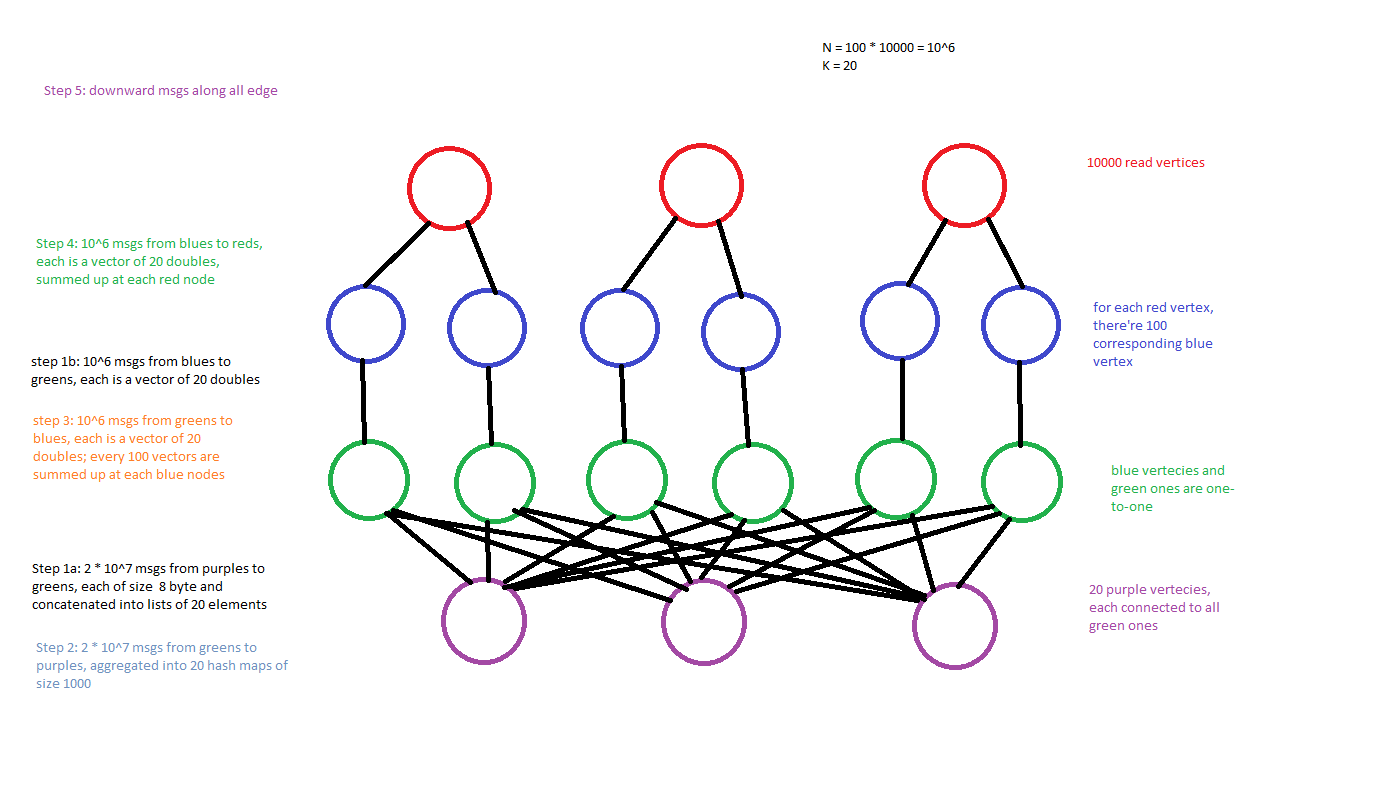
\includegraphics[scale=0.5]{lda.png}
%	\caption{Unrolled LDA bayesian network (TODO replace this with TSM)}
%\end{figure*}

